
%%%%%%%%%%%%%%%%%%%%%%%%%%%%%%%%%%%%%%%%%
% Jacobs Landscape Poster
% LaTeX Template
% Version 1.0 (29/03/13)
%
% Created by:
% Computational Physics and Biophysics Group, Jacobs University
% https://teamwork.jacobs-university.de:8443/confluence/display/CoPandBiG/LaTeX+Poster
% 
% Further modified by:
% Nathaniel Johnston (nathaniel@njohnston.ca)
%
% Modified further still by:
% Abraham Nunes (nunes <at> dal <dot> ca)
%
% License:
% CC BY-NC-SA 3.0 (http://creativecommons.org/licenses/by-nc-sa/3.0/)
%
%%%%%%%%%%%%%%%%%%%%%%%%%%%%%%%%%%%%%%%%%

%----------------------------------------------------------------------------------------
%	PACKAGES AND OTHER DOCUMENT CONFIGURATIONS
%----------------------------------------------------------------------------------------
\documentclass[final]{beamer}

\usepackage[scale=1]{beamerposter} % Use the beamerposter package for laying out the poster

\usetheme{confposter} % Use the confposter theme supplied with this template

\setbeamercolor{block title}{fg=black,bg=white} % Colors of the block titles
\setbeamercolor{block body}{fg=black,bg=white} % Colors of the body of blocks
\setbeamercolor{block alerted title}{fg=white,bg=erd} % Colors of the highlighted block titles
\setbeamercolor{block alerted body}{fg=black,bg=white} % Colors of the body of highlighted blocks
% Many more colors are available for use in beamerthemeconfposter.sty

%-----------------------------------------------------------
% Define the column widths and overall poster size
% To set effective sepwid, onecolwid and twocolwid values, first choose how many columns you want and how much separation you want between columns
% In this template, the separation width chosen is 0.024 of the paper width and a 4-column layout
% onecolwid should therefore be (1-(# of columns+1)*sepwid)/# of columns e.g. (1-(4+1)*0.024)/4 = 0.22
% Set twocolwid to be (2*onecolwid)+sepwid = 0.464
% Set threecolwid to be (3*onecolwid)+2*sepwid = 0.708
\usepackage[T2A]{fontenc}
\usepackage[utf8]{inputenc}	
\usepackage[english,russian]{babel}
\usepackage{mwe}
\usepackage{amsmath} 
\usepackage{mathtext} 
\usepackage{mathrsfs}
\usepackage{amsmath}
\usepackage{amsfonts}
\usepackage{amsthm}
\usepackage{amssymb}
\usepackage{mathrsfs}
\usepackage{mathtools}
\newlength{\sepwid}
\newlength{\onecolwid}
\newlength{\twocolwid}
\newlength{\threecolwid}
\setlength{\paperwidth}{48in} % A0 width: 46.8in
\setlength{\paperheight}{36in} % A0 height: 33.1in
\setlength{\sepwid}{0.024\paperwidth} % Separation width (white space) between columns
\setlength{\onecolwid}{0.22\paperwidth} % Width of one column
\setlength{\twocolwid}{0.464\paperwidth} % Width of two columns
\setlength{\threecolwid}{0.708\paperwidth} % Width of three columns
\setlength{\topmargin}{-0.5in} % Reduce the top margin size
%-----------------------------------------------------------

\usepackage{graphicx}  % Required for including images

\usepackage{booktabs} % Top and bottom rules for tables

%----------------------------------------------------------------------------------------
%	TITLE SECTION 
%----------------------------------------------------------------------------------------

\title{Энтропия} % Poster title

\author{Терверессы: Лиза, Олеся, Даша, Марина, Яна} % Author(s)
\titlegraphic{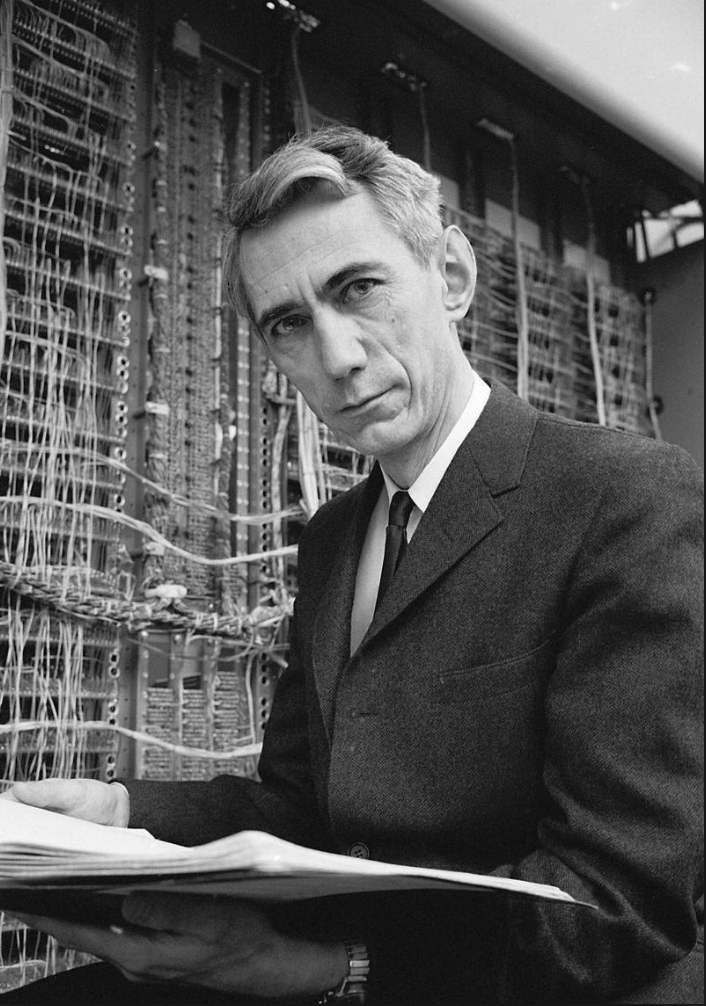
\includegraphics[scale=0.5]{klod.png}}
\institute{БЭК 171} % Institution(s)


%----------------------------------------------------------------------------------------
\usepackage{exscale}
\begin{document}

\addtobeamertemplate{block end}{}{\vspace*{2ex}} % White space under blocks
\addtobeamertemplate{block alerted end}{}{\vspace*{2ex}} % White space under highlighted (alert) blocks

\setlength{\belowcaptionskip}{2ex} % White space under figures
\setlength\belowdisplayshortskip{2ex} % White space under equations

\begin{frame}[t] % The whole poster is enclosed in one beamer frame

\begin{columns}[t] % The whole poster consists of three major columns, the second of which is split into two columns twice - the [t] option aligns each column's content to the top

\begin{column}{\sepwid}\end{column} % Empty spacer column

\begin{column}{\onecolwid} % The first column

%----------------------------------------------------------------------------------------
%	OBJECTIVES
%----------------------------------------------------------------------------------------

\setbeamercolor{block alerted title}{fg=white,bg=jblue} % Change the alert block title colors
\setbeamercolor{block alerted body}{fg=black,bg=white} % Change the alert block body colors

\begin{alertblock}{}
    \begin{itemize}
    \item 1948 год - Клод Шеннон создал первую, истинно математическую, теорию энтропии
	\item Его идеи послужили основой разработки двух основных направлений: теории информации и теории кодирования
    \end{itemize}
    
    \end{alertblock}
%----------------------------------------------------------------------------------------
%	INTRODUCTION
%----------------------------------------------------------------------------------------

\begin{block}{Для дискретных случайных величин}
\begin{itemize}
	\item \textbf{Энтропия} -- наименьшее среднее число бит, необходимое для кодирования некоторой информации.
    \[H=-\sum\limits_{i=1}^n p_i\log p_i, \]
    где $p_i$ --- вероятность $i$-го исхода    
    \item \textbf{Условная энтропия} --- количество бит, необходимое для того, чтобы узнать значение случайной величины $Y$ при условии, что случайная величина $X$ известна.
    \[H(Y|X)=-\sum\limits_{x, y} p(x, y)\log \cfrac{p(x, y)}{p(x)} \]
    \item \textbf{Совместная энтропия} --- степень неопределенности, связанная со множеством случайных величин.
    \[H(X, Y)=-\sum\limits_{x}\sum\limits_{y} p(x, y)\log p(x ,y) \]
    \item \textbf{Взаимная информация} $I(X; Y)$ --- мера взаимной зависимости двух случайных величин.
    \[I(X; Y) = \sum\limits_{x}\sum\limits_{y} p(x, y)\log \cfrac{p(x, y)}{p(x)p(y)} \]
\end{itemize}
\end{block}

\setbeamercolor{block alerted title}{fg=white,bg=jblue} % Change the alert block title colors
\setbeamercolor{block alerted body}{fg=black,bg=white} % Change the alert block body colors

\begin{alertblock}{Люблю решать задачки!}
	\begin{enumerate}
		\item Красная Шапочка встретила соседа-лесоруба Николая Петровича по дороге к бабушке Елене, которая равновероятно может жить в одной из трех деревень. Шапка точно помнит, в какой именно. Поскольку девочка маленькая, а неподалеку обитает волк, лесоруб решил узнать, в какой деревне живет бабушка, только не спросив напрямую, а задавая наводящие вопросы. 

		Найдите энтропию местонахождения Елены. 
	
		\item Оказалось, на дороге в одну из трёх деревень, в каждой из которых равновероятно может находиться бабуля Елена, ошивается злой волк Матвей, а в одну деревню ведет только одна дорога. Вероятности того, что Матвей находится в деревне $i$-той ($X$ --- местонахождение волка по вертикали), и того, что Елена в деревне $j$-той ($Y$ --- местонахождение бабули по горизонтали):
		\begin{center}
			\begin{tabular}{c||c|c|c}
				Деревня & 2112 & 2110 & К10 \\
				\hline
				\hline
				2112 & 1/4 & 1/24 & 1/24 \\
				\hline
				2110 & 1/24 & 1/4 & 1/24 \\
				\hline
				К10 & 1/24 & 1/24 & 1/4 \\
			\end{tabular}
		\end{center}
		
		Найдите совместную энтропию местонахождения Елены и Матвея: $H(X, Y)$. 
	\end{enumerate}
    
\end{alertblock}

%------------------------------------------------

%\begin{figure}
%\includegraphics[width=0.8\linewidth]{placeholder.jpg}
%\caption{Figure caption}
%\end{figure}

%----------------------------------------------------------------------------------------

\end{column} % End of the first column

\begin{column}{\sepwid}\end{column} % Empty spacer column

\begin{column}{\twocolwid} % Begin a column which is two columns wide (column 2)

\begin{columns}[t,totalwidth=\twocolwid] % Split up the two columns wide column

\begin{column}{\onecolwid}\vspace{-.6in} % The first column within column 2 (column 2.1)

%----------------------------------------------------------------------------------------
%	MATERIALS
%----------------------------------------------------------------------------------------



\begin{itemize}
	\item \textbf{Кросс энтропия} --- минимальное среднее количество бит, необходимое для того, чтобы закодировать информацию, если схема кодирования базируется на некотором распределении $q$, а не истинном, $p$.
	
	\[CE(P||Q)=-\sum\limits_{i=1}^{n}p_i\log q_i \]
	
	\item \textbf{Дивергенция Кульбака -- Лейблера} --- степень отдаленности одного вероятностного распределения от другого.
	
	\[D_{KL}(P\, ||\, Q)=  - \sum\limits_{i=1}^n p_i\log q_i\ - ( - \sum\limits_{i=1}^n p_i\log p_i)\]
\end{itemize}
	

\setbeamercolor{block alerted title}{fg=white,bg=jblue} % Change the alert block title colors
\setbeamercolor{block alerted body}{fg=black,bg=white} % Change the alert block body colors
\begin{alertblock}{Ещё задача :)}
	Красная Шапочка, убегая от злого лесоруба Николая Петровича, в панике перепутала вероятности, с которыми охотник Борис находится в одной из деревень ($X$ --- местонахождение охотника):
\[\begin{pmatrix}
    1/6 & 2/3 & 1/6
\end{pmatrix} , \] и с которыми волк Матвей ошивается на одной из дорог в деревни ($Y$ --- местонахождение волка):
\[\begin{pmatrix}
    3/8 & 3/8 & 1/4 
\end{pmatrix} .\]

(а) Найдите кросс-энтропию из истинного распределения местонахождения Матвея в распределение местонахождения Бориса;

(б) Вычислите дивергенцию Кульбака-Лейблера.
\end{alertblock}

\begin{block}{Для непрерывных случайных величин}

\begin{itemize}
	\item Самая главная и простая энтропийка:
	\[H(X)=-\int\limits_{-\infty}^{+\infty} f(x)\log f(x)dx \]
	\item Условная энтропия:
	\[H(Y|X)=-\int\limits_{-\infty}^{+\infty} f(x, y)\log f_{Y|X}(y)dy \]
	\item Совместная энтропия:
	\[H(X, Y)=-\int\limits_{-\infty}^{+\infty} \int\limits_{-\infty}^{+\infty} f(x, y)\log f(x, y)dxdy \]
	\item Взаимная информация:
	\[I(X; Y)=\int\limits_{-\infty}^{+\infty} \int\limits_{-\infty}^{+\infty} f(x, y) \log \cfrac{f(x, y)}{f(x)f(y)}dxdy \]
	\item Кросс-энтропия:
	\[CH(p, q)=-\int\limits_{-\infty}^{+\infty}p(x)\log q(x) dx \]
	\item Дивергенция Кульбака -- Лейблера:
	\begin{multline*}
		D_{KL}(P\, ||\, Q)=\int\limits_{-\infty}^{+\infty} p(x)\log p(x)dx -\int\limits_{-\infty}^{+\infty} p(x)\log q(x)dx
	\end{multline*}
\end{itemize}
\end{block}

%----------------------------------------------------------------------------------------

\end{column} % End of column 2.1

\begin{column}{\onecolwid}\vspace{-.6in} % The second column within column 2 (column 2.2)

%----------------------------------------------------------------------------------------
%	METHODS
%----------------------------------------------------------------------------------------
\setbeamercolor{block alerted title}{fg=white,bg=jblue} % Change the alert block title colors
\setbeamercolor{block alerted body}{fg=black,bg=white} % Change the alert block body colors
\begin{alertblock}{Задачи с абсолютно непрерывными случайными величинами}
	лрим
\end{alertblock}

\begin{block}{Энтропийное кодирование}
%\textbf{Энтропийное кодирование}

%\begin{figure}
%\includegraphics[width=0.8\linewidth]{placeholder.jpg}
%\caption{Figure caption}
%\end{figure}

Энтропия показывает наименьшее среднее число бит, необходимое для кодирования некоторой информации. С целью минимизации энтропии и оптимизации кода элементы с большой вероятностью появления кодируются меньшим числом символов. Это позволяет передавать большее количество информации, затрачивая меньший объем памяти.
\end{block}
\begin{block}{Построение решающих деревьев}
%\textbf{Построение решающих деревьев}

Каждое ветвление дерева представляет собой разделение выборки на две части по порогу некоторого признака. Расчет энтропии помогает определить оптимальный порог для каждого узла --- при котором взвешенная сумма энтропий получившихся выборок минимальна среди возможных разбиений.

Например, у нас есть выборка объектов с одним признаком, длина: обыкновенный удав (22 попугая), анаконда (46 попугаев), анаконда (40 попугаев), обыкновенный удав (31 попугай).

Попробуем разделить выборку по 38 попугаям (ОУ --- обыкновенный удав, А --- анаконда):
\begin{center}
	\tikzstyle{level 1}=[level distance=3cm, sibling distance=7cm]
	\tikzstyle{level 2}=[level distance=3cm, sibling distance=1cm]
	\tikz
	\node {Длина < 38 попугаев}
	child { node {Да}
		child { node {ОУ, ОУ}}}
	child { node {Нет}
		child { node {А, А}}};
\end{center}

При расчете энтропии $0 \cdot \log_2 0$ считается равным 0, несмотря на $\log_2 0$. За вероятность принимается вероятность встретить данный класс в новой выборке.

Энтропия левой части: $-(1 \cdot \log_2 1 + 0 \cdot \log_2 0) = 0$. Энтропия правой части: $-(1 \cdot \log_2 1 + 0 \cdot \log_2 0) = 0$. Суммарная энтропия получилась: $\frac{1}{2} \cdot 0 + \frac{1}{2} \cdot 0 = 0, \frac{1}{2}$ --- доля каждой выборки в исходной. 

Так как 0 --- минимально возможное значение энтропии, критерий <<длина < 38 попугаев>> дает оптимальный результат.
\end{block}


%----------------------------------------------------------------------------------------

\end{column} % End of column 2.2

\end{columns} % End of the split of column 2 - any content after this will now take up 2 columns width

%----------------------------------------------------------------------------------------
%	IMPORTANT RESULT
%----------------------------------------------------------------------------------------

\setbeamercolor{block alerted title}{fg=black,bg=dalgold} % Change the alert block title colors
\setbeamercolor{block alerted body}{fg=black,bg=white} % Change the alert block body colors

%----------------------------------------------------------------------------------------

\begin{columns}[t,totalwidth=\twocolwid] % Split up the two columns wide column again

\begin{column}{\onecolwid} % The first column within column 2 (column 2.1)

%----------------------------------------------------------------------------------------
%	MATHEMATICAL SECTION
%----------------------------------------------------------------------------------------

%----------------------------------------------------------------------------------------

\end{column} % End of column 2.1

\begin{column}{\onecolwid} % The second column within column 2 (column 2.2)

%----------------------------------------------------------------------------------------
%	RESULTS
%----------------------------------------------------------------------------------------



%----------------------------------------------------------------------------------------

\end{column} % End of column 2.2

\end{columns} % End of the split of column 2

\end{column} % End of the second column

\begin{column}{\sepwid}\end{column} % Empty spacer column

\begin{column}{\onecolwid} % The third column

%----------------------------------------------------------------------------------------
%	CONCLUSION
%----------------------------------------------------------------------------------------
\begin{block}{Применение в алгоритме UMAP}
	%\textbf{Применение в алгоритме UMAP}
	
	В анализе данных алгоритмы снижения размерности используют кросс-энтропию как показатель эффективности перенесения свойств объектов. Чем меньше кросс-энтропия, тем ближе к истинному оказалось подобранное отображение.

Приведем пример работы алгоритма UMAP. Мы возьмем набор данных об одежде, который включает в себя 70000 черно-белых изображений различной одежды по 10 классам: футболки, брюки, свитеры, платья, кроссовки и т.д. Каждая картинка имеет размер 28x28 пикселей или 784 пикселя.

Результатом преобразования будет следующее отображение:

\begin{figure}[!h]
	\noindent\centering{
		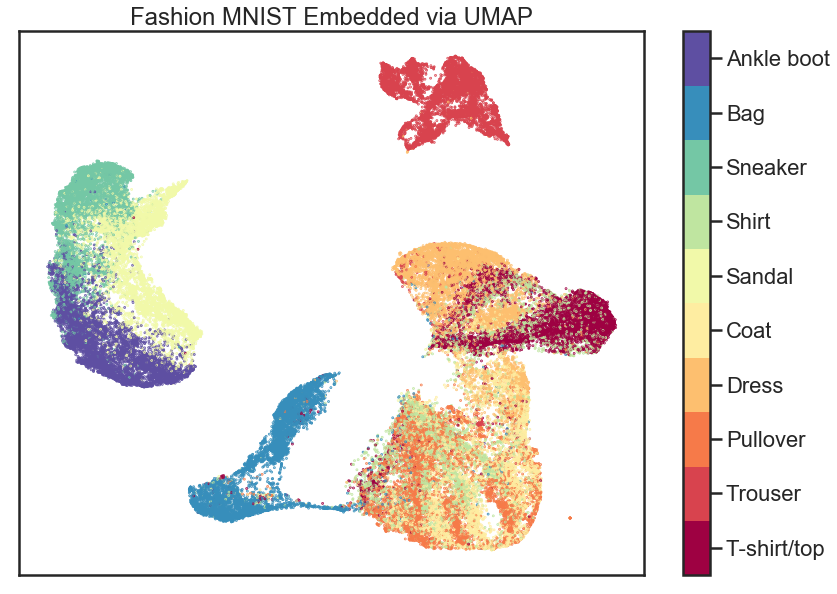
\includegraphics[height=9cm]{umap.png}
	}
	\caption{Алгоритм UMAP}
	\label{figCurves}
\end{figure} 

UMAP строит ориентированный взвешенный граф: ребрами соединяются каждый объект с наиболее похожими на него из выборки. Вес ребра можно интерпретировать как вероятность его существования. Тогда ребро $e$ является случайной величиной: $e \sim B(w(e))$. Множество ребер построенного графа --- множество $E$ из случайных величин Бернулли.

Чтобы перенести граф в низкоразмерное пространство, UMAP подбирает для множества~$E_h$ похожее на него множество~$E_l$ с функцией~$w_l(e)$, соответствующие низкоразмерному пространству

Для этого UMAP минимизирует сумму дивергенций Кульбака-Лейблера для каждой случайной величины из множеств:
\begin{multline*}
	S(E_h||E_l) = \sum_{e \in E} w_h(e) \log \frac{w_h(e)}{w_l(e)} + \\ + (1 - w_h(e)) \log \left(\frac{1 - w_h(e)}{1 - w_l(e)}\right) \rightarrow \min_{w_l}
\end{multline*}

Результатом является граф в низкоразмерном пространстве с подобранной функцией весов $w_l$.
\end{block}
%----------------------------------------------------------------------------------------
%	ADDITIONAL INFORMATION
%----------------------------------------------------------------------------------------

%----------------------------------------------------------------------------------------
%	ACKNOWLEDGEMENTS
%----------------------------------------------------------------------------------------

\setbeamercolor{block title}{fg=black,bg=white} % Change the block title color


%----------------------------------------------------------------------------------------
%	CONTACT INFORMATION
%----------------------------------------------------------------------------------------

\setbeamercolor{block alerted title}{fg=black,bg=dalblue} % Change the alert block title colors
\setbeamercolor{block alerted body}{fg=black,bg=white} % Change the alert block body colors

\begin{block}{Для тех, кто хочет больше!}

Воспользуйтесь qr-кодом и посмотрите полный текст повести про энтропию :)

\begin{center}
	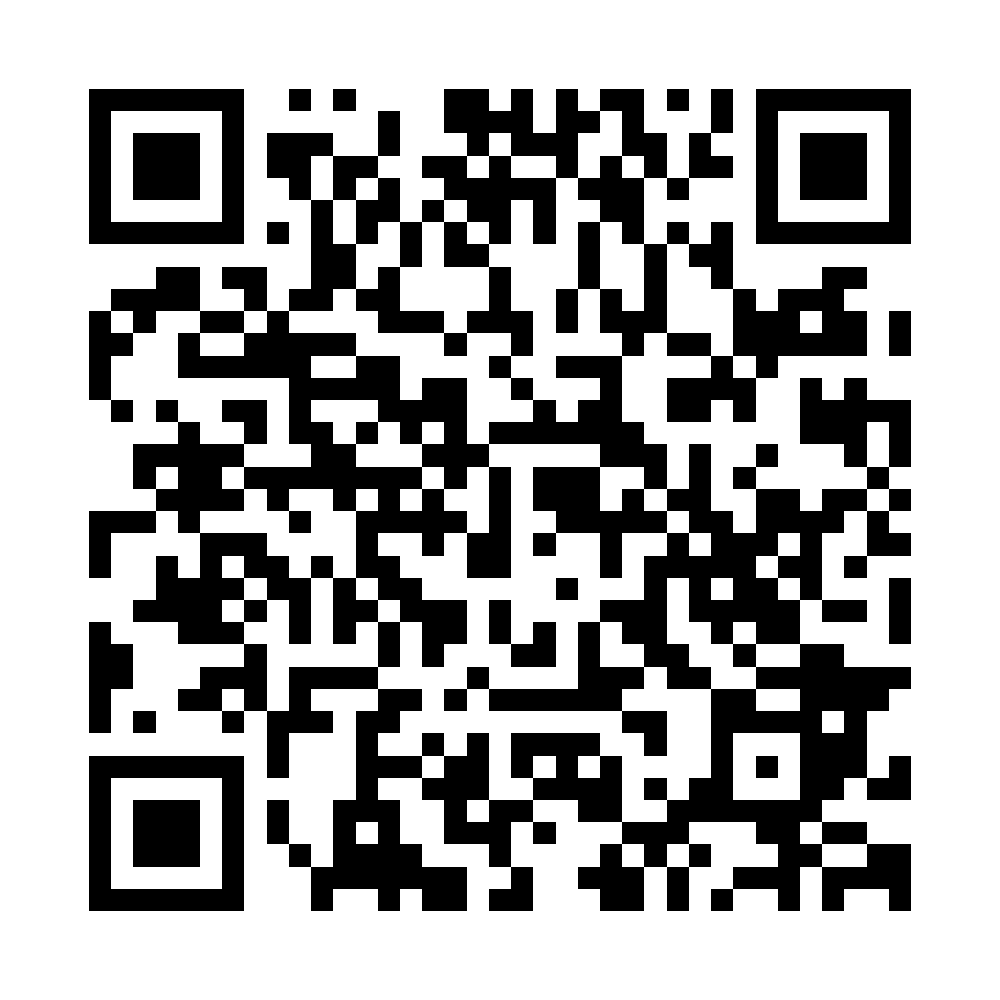
\includegraphics[scale=0.3]{qrcode.png}
\end{center}

\end{block}

%\begin{center}
%\includegraphics[width=0.8\linewidth]{dal_fullmark_blak.jpg}
%\end{center}
%----------------------------------------------------------------------------------------

\end{column} % End of the third column

\end{columns} % End of all the columns in the poster

\end{frame} % End of the enclosing frame

\end{document}